\setcounter{exo}{0}

On donne les équations du moteur à courant continu :
\begin{itemize}
\item $u(t) = e(t)+ Ri(t) +L \dfrac{\text{d}i(t)}{\text{d} t}$;
\item $e(t)=K\omega(t)$;
\item $c(t)=Ki(t)$;
\item $c(t)- f\omega(t)=J\dfrac{\text{d}\omega(t)}{\text{d} t}$.
\end{itemize}
\subparagraph{}
\textit{Réaliser le schéma-blocs.}

\ifprof
\begin{corrige}
\begin{center}
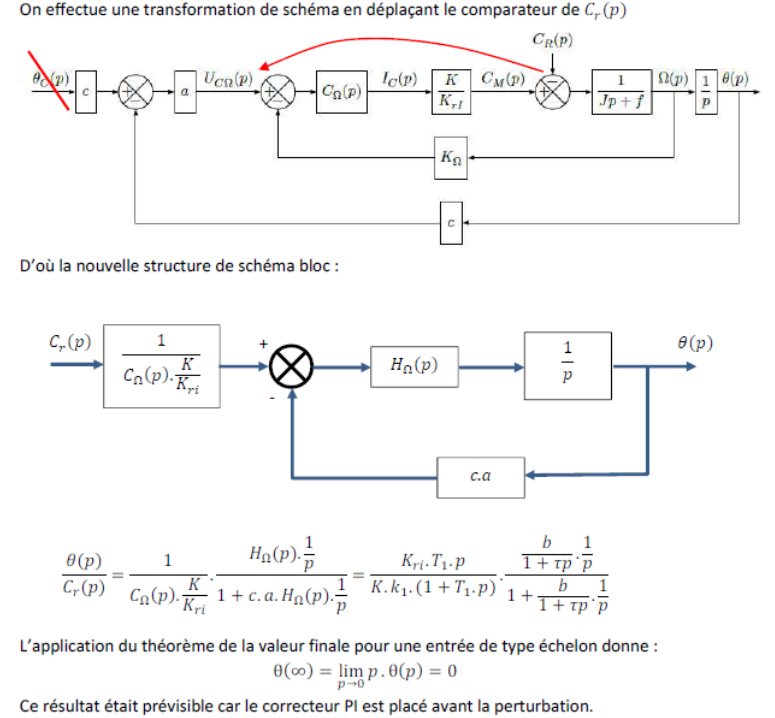
\includegraphics[width=.9\linewidth]{cor_01}
\end{center}
\end{corrige}
\else
\fi

\vspace{.5cm}

On donne le schéma de principe d'une servo-commande.
\begin{center}
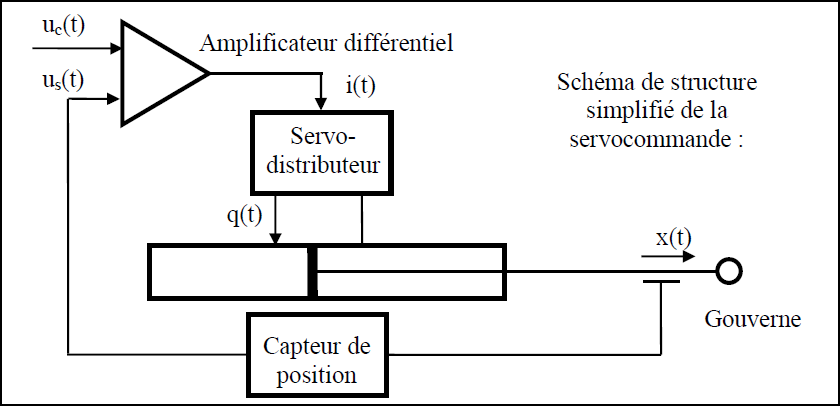
\includegraphics[width=.9\linewidth]{img5}
\end{center}

Les différentes équations temporelles qui modélisent le fonctionnement d'une servocommande sont :
\begin{itemize}
\item un amplificateur différentiel défini par : $u_c(t)=\dfrac{i(t)}{K_a}+u_s(t)$;
\item débit dans le vérin dans le cas d'une hypothèse de fluide incompressible $q(t)=S\cdot\dfrac{\dd x(t)}{\dd t}$;
\item capteur de position : $u_s(t)=K_c\cdot x(t)$;
\item le servo-distributeur est un composant de la chaîne de commande conçu pour fournir un débit hydraulique $q(t)$ proportionnel au courant de commande $i(t)$. (Attention, valable uniquement en régime permanent.) Le constructeur fournit sa fonction de transfert :
$$
F(p)=\dfrac{Q(p)}{I(p)}=\dfrac{K_d}{1+Tp}
$$
où $K_d$ est le gain du servo-distributeur et $T$ sa constante de temps.
\end{itemize}

\subparagraph{}
\textit{Réaliser le schéma-blocs.}
\ifprof
\begin{corrige}
On a :
\begin{itemize}
\item $U_c(p)=\dfrac{1}{K_a}I(p)+U_s(p)$
\item $Q(p)=SpX(p)$
\item $U_S(p)=K_C\cdot X(p)$
\item $F(p)=\dfrac{Q(p)}{I(p)}=\dfrac{K_d}{1+Tp}$
\end{itemize}


\begin{minipage}[c]{.23\linewidth}
\begin{center}
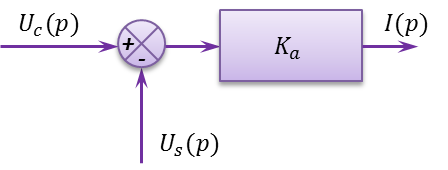
\includegraphics[width=.95\textwidth]{bloc1}
\end{center}
\end{minipage}\hfill
\begin{minipage}[c]{.23\linewidth}
\begin{center}
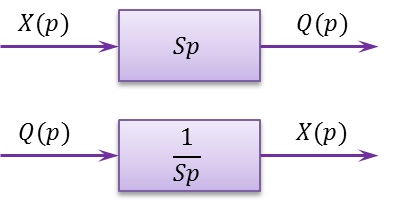
\includegraphics[width=.95\textwidth]{bloc2}
\end{center}
\end{minipage}\hfill
\begin{minipage}[c]{.23\linewidth}
\begin{center}
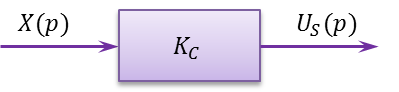
\includegraphics[width=.95\textwidth]{bloc3}
\end{center}
\end{minipage}\hfill
\begin{minipage}[c]{.23\linewidth}
\begin{center}
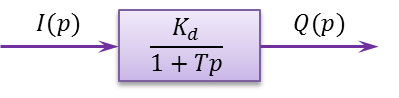
\includegraphics[width=.95\textwidth]{bloc4}
\end{center}
\end{minipage}



\begin{center}
\includegraphics[width=.8\textwidth]{schema_bloc}
\end{center}
\end{corrige}
\else 
\fi
